\tikzset{every picture/.style={line width=1.75pt}} %set default line width to 0.75pt        

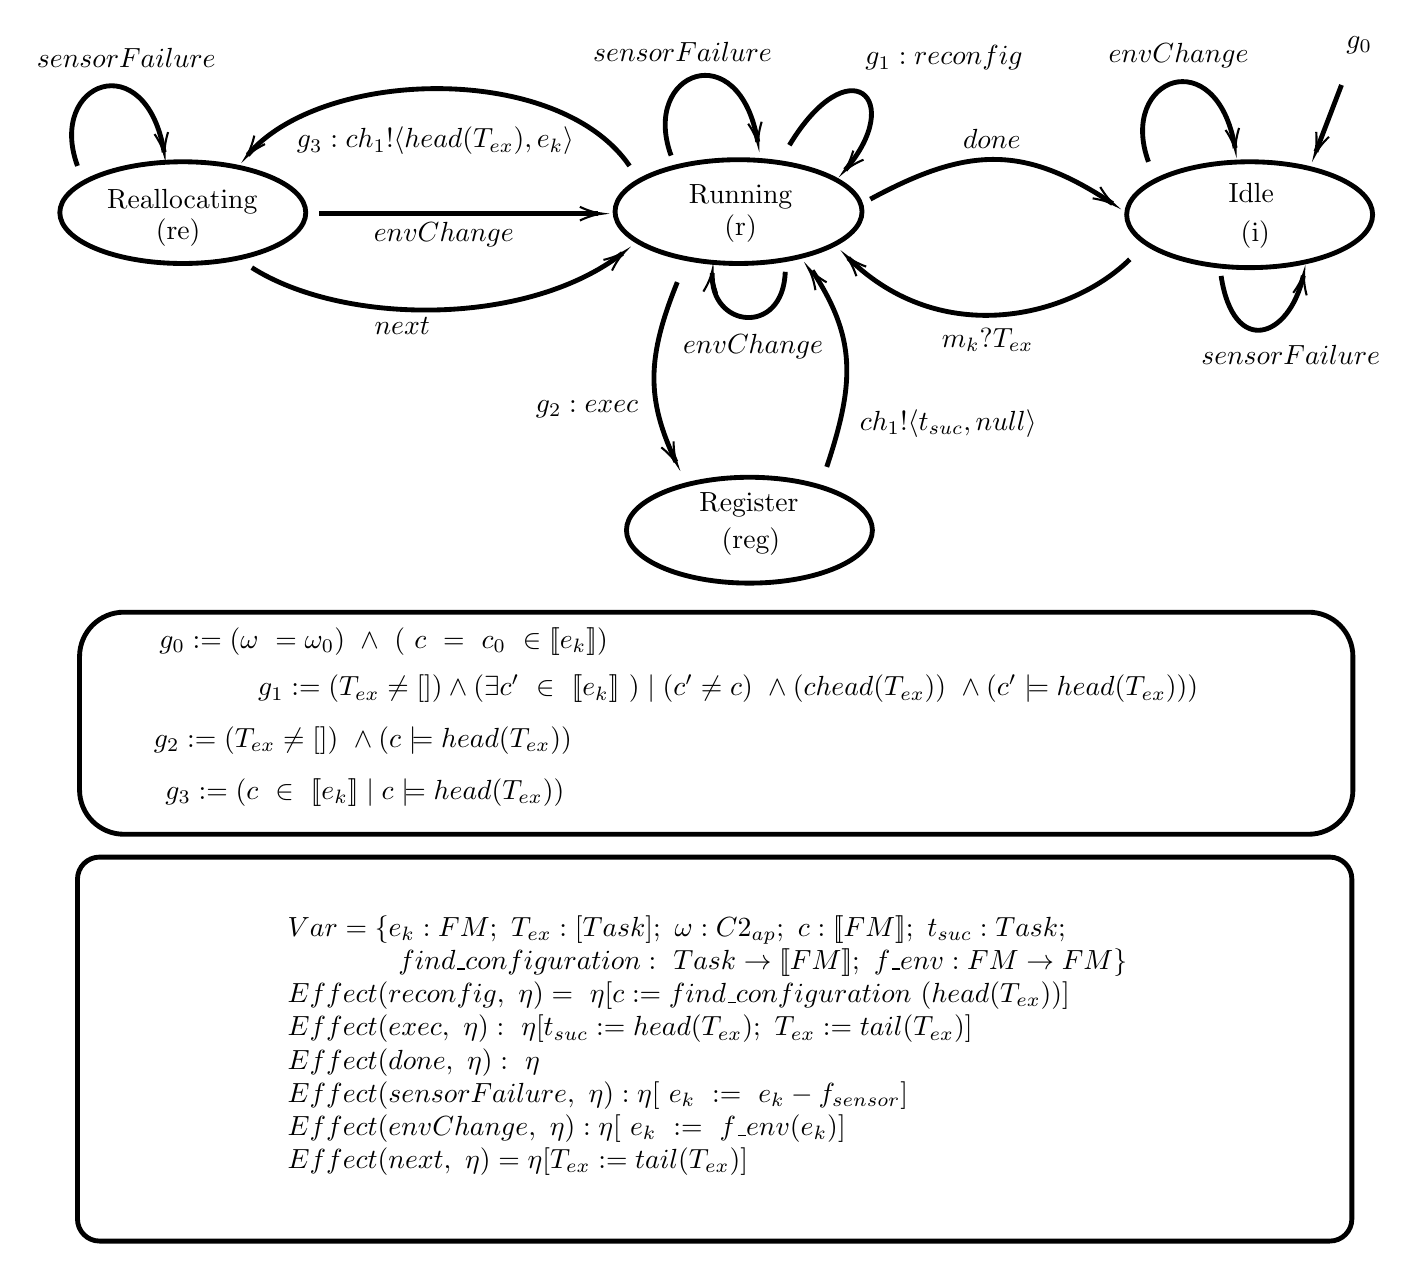
\begin{tikzpicture}[x=0.75pt,y=0.75pt,yscale=-1,xscale=1]
%uncomment if require: \path (0,606); %set diagram left start at 0, and has height of 606

%Curve Lines [id:da9480858267519683] 
\draw    (385.5,222) .. controls (399.29,180.63) and (399.5,159.63) .. (378.52,127.48) ;
\draw [shift={(376.5,126)}, rotate = 415.12] [color={rgb, 255:red, 0; green, 0; blue, 0 }  ][line width=0.75]    (10.93,-3.29) .. controls (6.95,-1.4) and (3.31,-0.3) .. (0,0) .. controls (3.31,0.3) and (6.95,1.4) .. (10.93,3.29)   ;
%Shape: Ellipse [id:dp6594609066072359] 
\draw   (283.5,99) .. controls (283.5,85.19) and (310.14,74) .. (343,74) .. controls (375.86,74) and (402.5,85.19) .. (402.5,99) .. controls (402.5,112.81) and (375.86,124) .. (343,124) .. controls (310.14,124) and (283.5,112.81) .. (283.5,99) -- cycle ;
%Shape: Ellipse [id:dp873836537729809] 
\draw   (530,100.5) .. controls (530,86.42) and (556.53,75) .. (589.25,75) .. controls (621.97,75) and (648.5,86.42) .. (648.5,100.5) .. controls (648.5,114.58) and (621.97,126) .. (589.25,126) .. controls (556.53,126) and (530,114.58) .. (530,100.5) -- cycle ;
%Curve Lines [id:da21020703050779688] 
\draw    (367.5,67) .. controls (396.21,19.48) and (423.94,44.49) .. (394.41,78.95) ;
\draw [shift={(393.5,80)}, rotate = 311.53] [color={rgb, 255:red, 0; green, 0; blue, 0 }  ][line width=0.75]    (10.93,-3.29) .. controls (6.95,-1.4) and (3.31,-0.3) .. (0,0) .. controls (3.31,0.3) and (6.95,1.4) .. (10.93,3.29)   ;
%Straight Lines [id:da37650774099478246] 
\draw    (633.5,38) -- (621.21,70.13) ;
\draw [shift={(620.5,72)}, rotate = 290.92] [color={rgb, 255:red, 0; green, 0; blue, 0 }  ][line width=0.75]    (10.93,-3.29) .. controls (6.95,-1.4) and (3.31,-0.3) .. (0,0) .. controls (3.31,0.3) and (6.95,1.4) .. (10.93,3.29)   ;
%Shape: Ellipse [id:dp02234558999259495] 
\draw   (16,99.5) .. controls (16,85.97) and (42.53,75) .. (75.25,75) .. controls (107.97,75) and (134.5,85.97) .. (134.5,99.5) .. controls (134.5,113.03) and (107.97,124) .. (75.25,124) .. controls (42.53,124) and (16,113.03) .. (16,99.5) -- cycle ;
%Curve Lines [id:da2517277021570281] 
\draw    (290.5,77) .. controls (255.85,26.51) and (141.81,29.93) .. (106.54,71.72) ;
\draw [shift={(105.5,73)}, rotate = 308.33000000000004] [color={rgb, 255:red, 0; green, 0; blue, 0 }  ][line width=0.75]    (10.93,-3.29) .. controls (6.95,-1.4) and (3.31,-0.3) .. (0,0) .. controls (3.31,0.3) and (6.95,1.4) .. (10.93,3.29)   ;
%Curve Lines [id:da851947022127026] 
\draw    (108.5,126) .. controls (152.06,153.72) and (240.7,154.98) .. (287.11,119.1) ;
\draw [shift={(288.5,118)}, rotate = 501.19] [color={rgb, 255:red, 0; green, 0; blue, 0 }  ][line width=0.75]    (10.93,-3.29) .. controls (6.95,-1.4) and (3.31,-0.3) .. (0,0) .. controls (3.31,0.3) and (6.95,1.4) .. (10.93,3.29)   ;
%Curve Lines [id:da05773774536505705] 
\draw    (531.5,122) .. controls (503.29,149.72) and (440.77,165.68) .. (395.86,121.36) ;
\draw [shift={(394.5,120)}, rotate = 405.63] [color={rgb, 255:red, 0; green, 0; blue, 0 }  ][line width=0.75]    (10.93,-3.29) .. controls (6.95,-1.4) and (3.31,-0.3) .. (0,0) .. controls (3.31,0.3) and (6.95,1.4) .. (10.93,3.29)   ;
%Rounded Rect [id:dp5913972444482631] 
\draw   (25.5,313.4) .. controls (25.5,301.58) and (35.08,292) .. (46.9,292) -- (617.6,292) .. controls (629.42,292) and (639,301.58) .. (639,313.4) -- (639,377.6) .. controls (639,389.42) and (629.42,399) .. (617.6,399) -- (46.9,399) .. controls (35.08,399) and (25.5,389.42) .. (25.5,377.6) -- cycle ;
%Rounded Rect [id:dp9206164489184118] 
\draw   (24.5,420.63) .. controls (24.5,414.76) and (29.26,410) .. (35.13,410) -- (627.88,410) .. controls (633.74,410) and (638.5,414.76) .. (638.5,420.63) -- (638.5,584.38) .. controls (638.5,590.24) and (633.74,595) .. (627.88,595) -- (35.13,595) .. controls (29.26,595) and (24.5,590.24) .. (24.5,584.38) -- cycle ;
%Curve Lines [id:da46585089178877326] 
\draw    (24.5,77) .. controls (9.65,36.41) and (57.53,18.36) .. (66.25,70.4) ;
\draw [shift={(66.5,72)}, rotate = 261.57] [color={rgb, 255:red, 0; green, 0; blue, 0 }  ][line width=0.75]    (10.93,-3.29) .. controls (6.95,-1.4) and (3.31,-0.3) .. (0,0) .. controls (3.31,0.3) and (6.95,1.4) .. (10.93,3.29)   ;
%Curve Lines [id:da24525569786800605] 
\draw    (575.5,130) .. controls (581.38,169.2) and (608.39,160.38) .. (615.11,129.89) ;
\draw [shift={(615.5,128)}, rotate = 460.62] [color={rgb, 255:red, 0; green, 0; blue, 0 }  ][line width=0.75]    (10.93,-3.29) .. controls (6.95,-1.4) and (3.31,-0.3) .. (0,0) .. controls (3.31,0.3) and (6.95,1.4) .. (10.93,3.29)   ;
%Curve Lines [id:da5617910694928671] 
\draw    (310.5,72) .. controls (295.65,31.41) and (343.53,13.36) .. (352.25,65.4) ;
\draw [shift={(352.5,67)}, rotate = 261.57] [color={rgb, 255:red, 0; green, 0; blue, 0 }  ][line width=0.75]    (10.93,-3.29) .. controls (6.95,-1.4) and (3.31,-0.3) .. (0,0) .. controls (3.31,0.3) and (6.95,1.4) .. (10.93,3.29)   ;
%Shape: Ellipse [id:dp893416141673501] 
\draw   (289,252.5) .. controls (289,238.42) and (315.53,227) .. (348.25,227) .. controls (380.97,227) and (407.5,238.42) .. (407.5,252.5) .. controls (407.5,266.58) and (380.97,278) .. (348.25,278) .. controls (315.53,278) and (289,266.58) .. (289,252.5) -- cycle ;
%Curve Lines [id:da2982425830385871] 
\draw    (313.5,133) .. controls (298.72,169.45) and (298.5,189.4) .. (312.84,219.61) ;
\draw [shift={(313.5,221)}, rotate = 244.18] [color={rgb, 255:red, 0; green, 0; blue, 0 }  ][line width=0.75]    (10.93,-3.29) .. controls (6.95,-1.4) and (3.31,-0.3) .. (0,0) .. controls (3.31,0.3) and (6.95,1.4) .. (10.93,3.29)   ;
%Curve Lines [id:da08998093824564413] 
\draw    (406.5,93) .. controls (454.02,67.26) and (480.96,67) .. (523.21,95.14) ;
\draw [shift={(524.5,96)}, rotate = 214] [color={rgb, 255:red, 0; green, 0; blue, 0 }  ][line width=0.75]    (10.93,-3.29) .. controls (6.95,-1.4) and (3.31,-0.3) .. (0,0) .. controls (3.31,0.3) and (6.95,1.4) .. (10.93,3.29)   ;
%Curve Lines [id:da7980176061132549] 
\draw    (365.5,128) .. controls (364.52,159.36) and (328.97,155.19) .. (330.37,128.65) ;
\draw [shift={(330.5,127)}, rotate = 456.12] [color={rgb, 255:red, 0; green, 0; blue, 0 }  ][line width=0.75]    (10.93,-3.29) .. controls (6.95,-1.4) and (3.31,-0.3) .. (0,0) .. controls (3.31,0.3) and (6.95,1.4) .. (10.93,3.29)   ;
%Curve Lines [id:da863076595467461] 
\draw    (540.5,75) .. controls (525.65,34.41) and (573.53,16.36) .. (582.25,68.4) ;
\draw [shift={(582.5,70)}, rotate = 261.57] [color={rgb, 255:red, 0; green, 0; blue, 0 }  ][line width=0.75]    (10.93,-3.29) .. controls (6.95,-1.4) and (3.31,-0.3) .. (0,0) .. controls (3.31,0.3) and (6.95,1.4) .. (10.93,3.29)   ;
%Straight Lines [id:da7258762513235244] 
\draw    (141,100) -- (275.5,100) ;
\draw [shift={(277.5,100)}, rotate = 180] [color={rgb, 255:red, 0; green, 0; blue, 0 }  ][line width=0.75]    (10.93,-3.29) .. controls (6.95,-1.4) and (3.31,-0.3) .. (0,0) .. controls (3.31,0.3) and (6.95,1.4) .. (10.93,3.29)   ;

% Text Node
\draw (344,92) node   [align=left] {Running};
% Text Node
\draw (590,90) node   [align=left] {Idle};
% Text Node
\draw (197,65) node    {$g_{3} :ch_{1} !\langle head( T_{ex}) ,e_{k} \rangle $};
% Text Node
\draw (463,161) node    {$m_{k} ?T_{ex}$};
% Text Node
\draw (75,94) node   [align=left] {Reallocating};
% Text Node
\draw (181,154) node    {$next$};
% Text Node
\draw (338,329) node    {$g_{1} :=( T_{ex} \neq []) \land ( \exists c'\ \in \ [\![ e_{k} ]\!] \ ) \mid ( c'\neq c) \ \land ( c\nvDash head( T_{ex})) \ \land ( c'\models head( T_{ex})))$};
% Text Node
\draw (442,25) node    {$g_{1} :reconfig$};
% Text Node
\draw (270,194) node    {$g_{2} :exec$};
% Text Node
\draw (162,354) node    {$g_{2} :=( T_{ex} \neq []) \ \land ( c\models head( T_{ex}))$};
% Text Node
\draw (232,455) node    {$ \begin{array}{l}
\end{array}$};
% Text Node
\draw (328,501) node    {$ \begin{array}{l}
Var=\{e_{k} :FM;\ T_{ex} :[ Task] ;\ \omega :C2_{ap} ;\ c:[\![ FM]\!] ;\ t_{suc} :Task;\ \\
\ \ \ \ \ \ \ \ \ \ \ \ find\_configuration:\ Task\rightarrow [\![ FM]\!] ;\ f\_env:FM\rightarrow FM\}\\
Effect( reconfig,\ \eta ) =\ \eta [ c:=find\_configuration\ ( head( T_{ex}))]\\
Effect( exec,\ \eta ) :\ \eta [ t_{suc} :=head( T_{ex}) ;\ T_{ex} :=tail( T_{ex})]\\
Effect( done,\ \eta ) :\ \eta \\
Effect( sensorFailure,\ \eta ) :\eta [ \ e_{k} \ :=\ e_{k} -f_{sensor}]\\
Effect( envChange,\ \eta ) :\eta [ \ e_{k} \ :=\ f\_env( e_{k})]\\
Effect( next,\ \eta ) =\eta [ T_{ex} :=tail( T_{ex})]
\end{array}$};
% Text Node
\draw (73,109) node   [align=left] {(re)};
% Text Node
\draw (344,107) node   [align=left] {(r)};
% Text Node
\draw (592,110) node   [align=left] {(i)};
% Text Node
\draw (642,19) node    {$g_{0}$};
% Text Node
\draw (163,379) node    {$g_{3} :=( \nexists c\ \in \ [\![ e_{k} ]\!] \mid c\models head( T_{ex}))$};
% Text Node
\draw (172,306) node    {$g_{0} :=( \omega \ =\omega _{0}) \ \land \ ( \ c\ =\ c_{0} \ \in [\![ e_{k} ]\!] )$};
% Text Node
\draw (48,25) node    {$sensorFailure$};
% Text Node
\draw (609,168) node    {$sensorFailure$};
% Text Node
\draw (465,64) node    {$done$};
% Text Node
\draw (316,22) node    {$sensorFailure$};
% Text Node
\draw (348,240) node   [align=left] {Register};
% Text Node
\draw (349,258) node   [align=left] {(reg)};
% Text Node
\draw (444,201) node    {$ch_{1} !\langle t_{suc} ,null\rangle $};
% Text Node
\draw (201,110) node    {$envChange$};
% Text Node
\draw (350,164) node    {$envChange$};
% Text Node
\draw (555,24) node    {$envChange$};


\end{tikzpicture}